\documentclass[a4paper,11pt]{article}

\usepackage[utf8]{inputenc}
\usepackage[T1]{fontenc}
\usepackage[brazil]{babel}
\usepackage{geometry}
\usepackage{setspace}
\usepackage{amsmath, amssymb, amsfonts}
\usepackage{booktabs}
\usepackage{array}
\usepackage{multirow}
\usepackage{graphicx}
\usepackage{float}
\usepackage{subcaption}
\usepackage[hidelinks]{hyperref}

\geometry{top=1.0cm, bottom=1.8cm, left=1.8cm, right=1.8cm}
\onehalfspacing

\graphicspath{{../figures/}}

\title{\textbf{Relatório T3} \\ \large MC906: Redes Neurais do Zero com Interpretabilidade}
\author{
    Adriano Ribeiro Franulovic Campos,
    Andrei Quaresma Pinto,
    Matheus Ferracciú Scatolin,\\
    Pietro Fernandes Magaldi,
    Tiago Perrupato Antunes\\
}
\date{Maio/2026}

\begin{document}
\maketitle

\begin{abstract}
Implementamos uma rede neural multicamadas (MLP) \emph{100\% NumPy} para classificar tumores do dataset \emph{Breast Cancer Wisconsin (Diagnostic)} em benignos ou malignos. O trabalho cobre forward pass, backpropagation e mini-batch SGD com ReLU, Softmax e cross-entropy; exploração de hiperparâmetros; avaliação final com early stopping; e interpretabilidade por gradientes de entrada e ablação. O melhor modelo alcançou \textbf{98,2\%} de acurácia no conjunto de teste (114 amostras), com dois erros.
\end{abstract}

\section{Introdução}

O diagnóstico precoce de câncer de mama depende de características morfológicas dos núcleos celulares extraídas de imagens histopatológicas. O dataset \emph{Breast Cancer Wisconsin (Diagnostic)}~\cite{sklearn-bc} disponibiliza 569 amostras com 30 atributos numéricos por tumor (médias, piores valores e erros de medidas como raio, textura, concavidade etc.) e rótulo binário.

\textbf{Objetivo do TP:} construir do zero uma MLP capaz de classificar tumores, compreender o aprendizado via retropropagação e \emph{explicar} as decisões do modelo. Não utilizamos PyTorch, TensorFlow ou bibliotecas equivalentes para o treinamento; apenas NumPy para a rede e scikit-learn para carregamento de dados, métricas auxiliares e comparação opcional.

\textbf{Pré-processamento.} Invertemos o encoding do scikit-learn para adotar B=0 (benigno) e M=1 (maligno). Aplicamos \emph{split} estratificado 64/16/20\% (363 treino, 91 validação, 115 teste), preservando a proporção de classes ($\approx$62,7\% benignos). Cada feature recebe z-score com média e desvio \emph{calculados apenas no treino}, evitando vazamento de informação. Para treino usamos \emph{one-hot encoding} dos rótulos, compatível com Softmax + cross-entropy.

A Figura~\ref{fig:pca} mostra projeção PCA 2D do teste: as classes são parcialmente separáveis, com região de sobreposição onde erros são mais prováveis.

\begin{figure}[H]
    \centering
    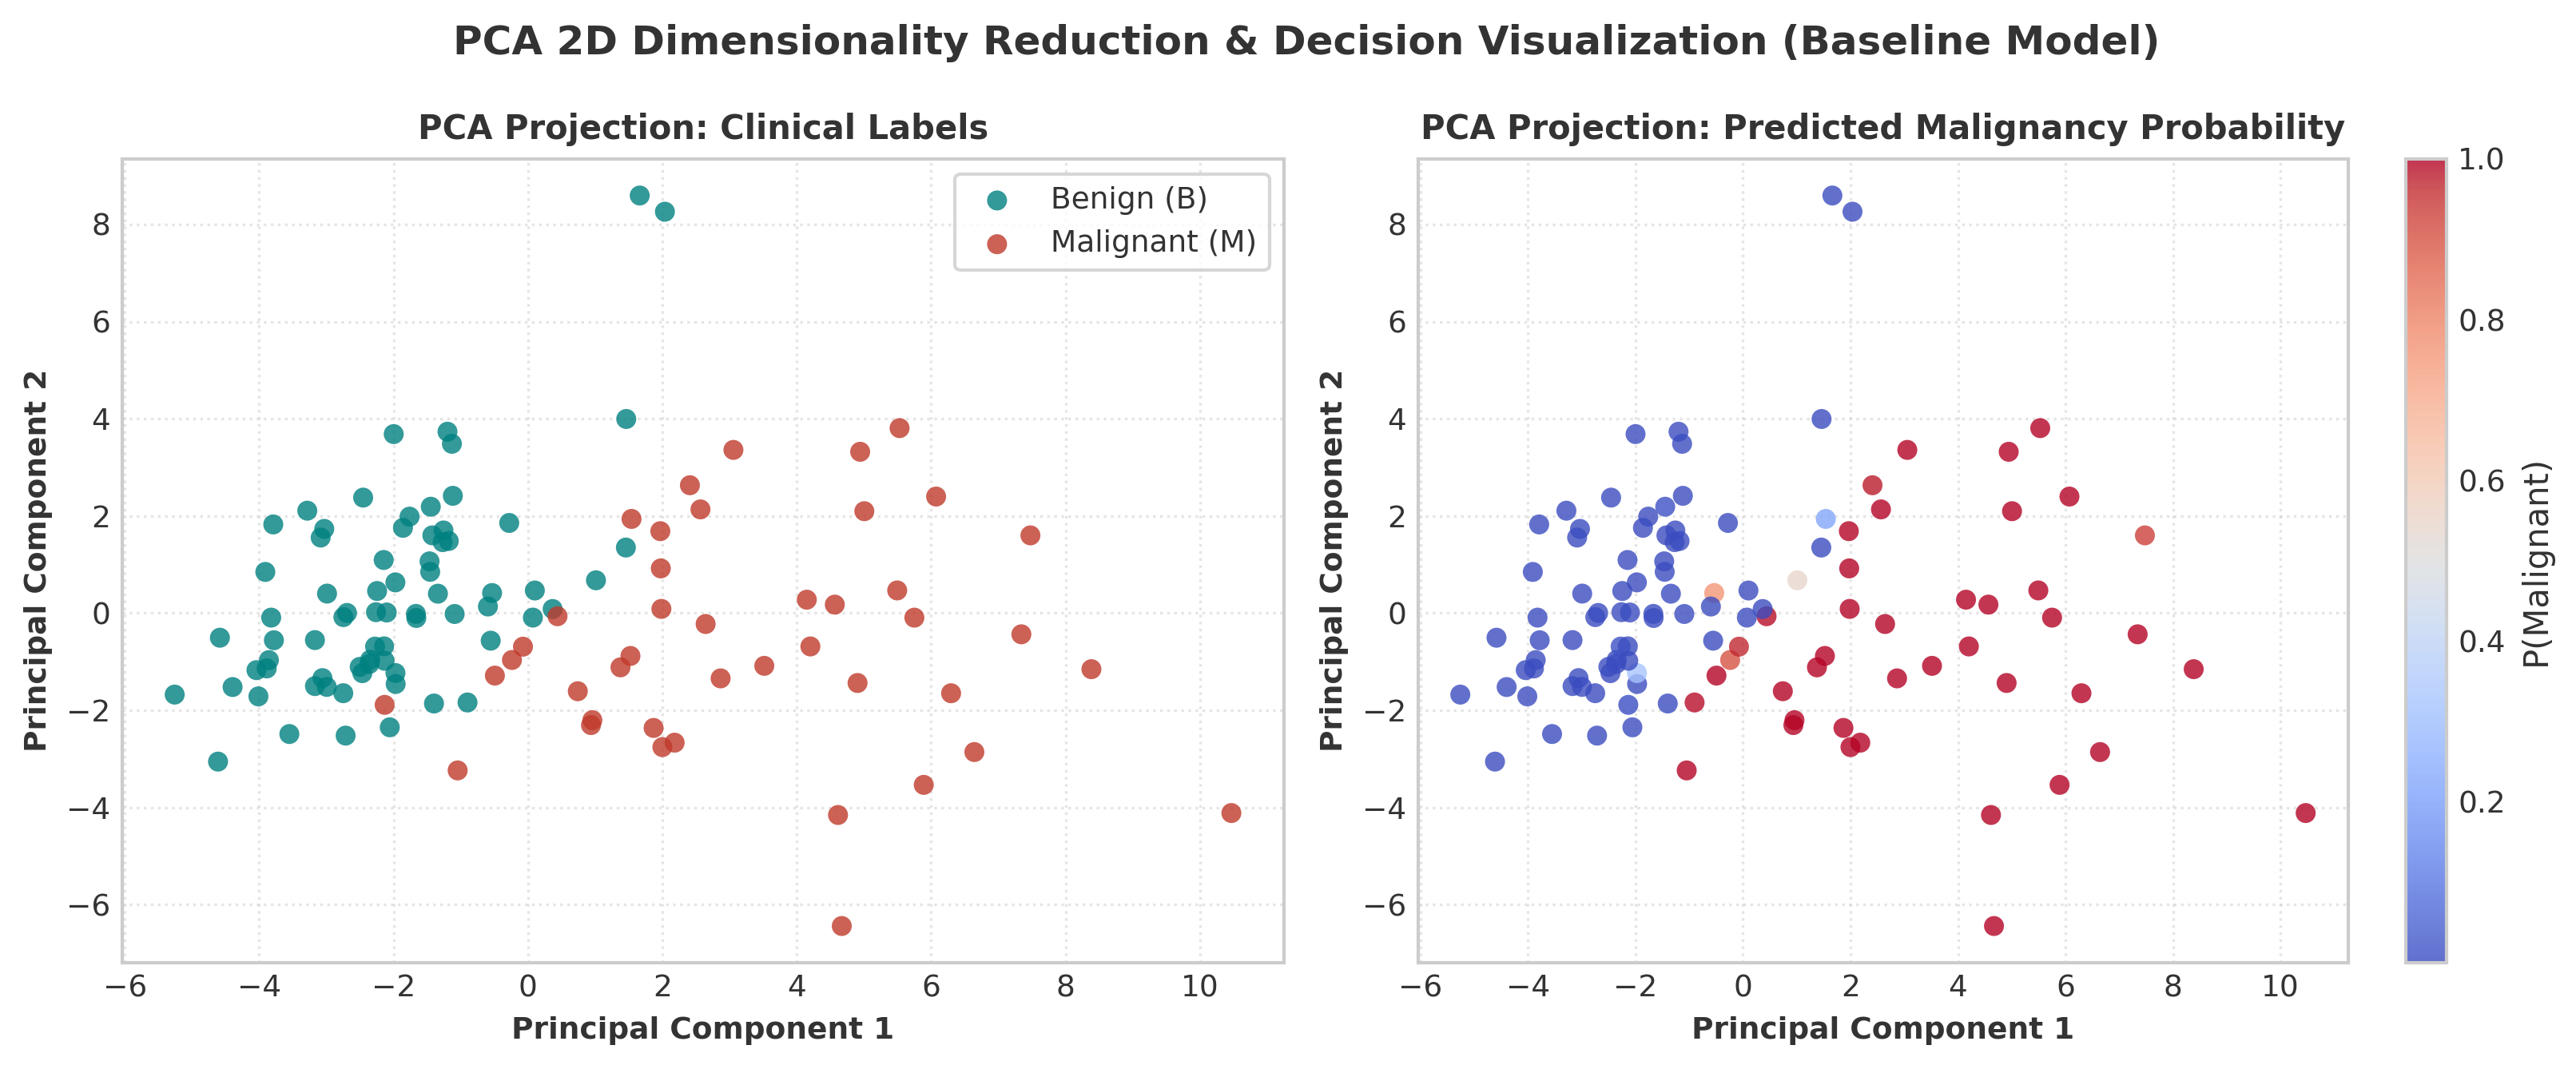
\includegraphics[width=0.85\linewidth]{pca_2d_projection_baseline.png}
    \caption{Projeção PCA 2D do conjunto de teste (esquerda: rótulos reais; direita: $P(\text{maligno})$ do modelo \emph{baseline}).}
    \label{fig:pca}
\end{figure}

\section{Implementação}

\subsection{Arquitetura}

A rede é totalmente conectada com $L$ camadas definidas por uma lista de tamanhos, e.g.\ \texttt{[30, 16, 2]}: 30 entradas, 16 neurônios ReLU na camada oculta e 2 logits de saída. Para cada camada $l$:
\begin{equation}
    \mathbf{z}^{(l)} = \mathbf{W}^{(l)} \mathbf{a}^{(l-1)} + \mathbf{b}^{(l)}, \qquad
    \mathbf{a}^{(l)} = \mathrm{ReLU}(\mathbf{z}^{(l)}) \quad (l < L),
\end{equation}
com $\mathbf{a}^{(0)} = \mathbf{x}$. Na saída aplicamos Softmax explícita:
\begin{equation}
    p_i = \frac{e^{z_i}}{\sum_j e^{z_j}}.
\end{equation}

\subsection{Função de custo e retropropagação}

Usamos cross-entropy multiclasse com rótulos \emph{one-hot} $\mathbf{y}$:
\begin{equation}
    \mathcal{L} = -\frac{1}{B}\sum_{b=1}^{B}\sum_{i} y_{bi}\,\log p_{bi}.
\end{equation}
Combinando Softmax + CE, o gradiente na saída simplifica-se a $(\mathbf{p} - \mathbf{y})/B$, propagado pelas camadas ocultas via regra da cadeia e gradiente da ReLU:
$\partial a / \partial z = \mathbb{1}[z > 0]$.

\subsection{Otimização}

Parâmetros atualizados por mini-batch SGD; opcionalmente com \textbf{momentum} $\mu$:
$\mathbf{v} \leftarrow \mu \mathbf{v} - \alpha \nabla \mathcal{L}$, $\theta \leftarrow \theta + \mathbf{v}$.
Implementamos também inicialização \textbf{He} para camadas ReLU ($\mathcal{N}(0,\, \sqrt{2/n_{\text{in}}})$). Pesos padrão usam $\mathcal{N}(0, 0.01)$ e vieses zero. Validamos a implementação com \emph{gradient check} numérico (erro $< 10^{-6}$).

\section{Experimentos}

\subsection{Metodologia}

\textbf{Métricas:} acurácia e loss de cross-entropy. Hiperparâmetros são selecionados pela \textbf{acurácia de validação} (média de 5 \emph{seeds}); o teste é usado \textbf{uma única vez} após a escolha final (Seção~5). Em empates de validação, mantemos a configuração mais simples.

\textbf{Baseline} (Seção~3): \texttt{arch=[30,32,2]}, $\alpha=0{,}1$, \texttt{batch=32}, 150 épocas, 3 \emph{seeds}. Converge rapidamente ($\approx$97 a 98\% val acc), com leve \emph{overfitting} após a época~15 (val loss sobe enquanto treino continua caindo; ver notebook, Figura~baseline).

\subsection{Exploração de hiperparâmetros}

Variamos \textbf{um hiperparâmetro por vez} (100 épocas, \emph{seeds} 1, 2, 42, 100, 2026). A Tabela~\ref{tab:hyper} resume os resultados.

\begin{table}[H]
    \centering
    \caption{Exploração de hiperparâmetros (100 épocas, 5 \emph{seeds}; varia-se um parâmetro por vez).}
    \label{tab:hyper}
    \small
    \begin{tabular}{llccc}
        \toprule
        Parâmetro & Valor & Train acc & Val acc & Val loss \\
        \midrule
        \multirow{3}{*}{$\alpha$} & 0{,}001 & 0{,}628 & 0{,}626 & 0{,}658 \\
        & 0{,}01  & 0{,}986 & \textbf{0{,}978} & 0{,}064 \\
        & 0{,}1   & 1{,}000 & 0{,}967 & 0{,}009 \\
        \midrule
        \multirow{3}{*}{Batch} & 8  & 0{,}992 & \textbf{0{,}978} & 0{,}024 \\
        & 32 & 0{,}986 & 0{,}978 & 0{,}064 \\
        & 64 & 0{,}964 & 0{,}967 & 0{,}141 \\
        \midrule
        \multirow{3}{*}{Arch} & \texttt{[30,16,2]}    & 0{,}992 & \textbf{0{,}978} & 0{,}025 \\
        & \texttt{[30,32,2]}    & 0{,}992 & 0{,}978 & 0{,}024 \\
        & \texttt{[30,64,32,2]} & 0{,}995 & 0{,}978 & 0{,}027 \\
        \bottomrule
    \end{tabular}
\end{table}

\textbf{Melhor configuração:} \texttt{arch=[30,16,2]}, $\alpha=0{,}01$, \texttt{batch=8} (val acc 0{,}978; escolhida por parsimônia ante empate). $\alpha=0{,}001$ permanece no patamar da classe majoritária ($\approx$0{,}63), indicando \emph{underfitting} severo.

\begin{figure}[H]
    \centering
    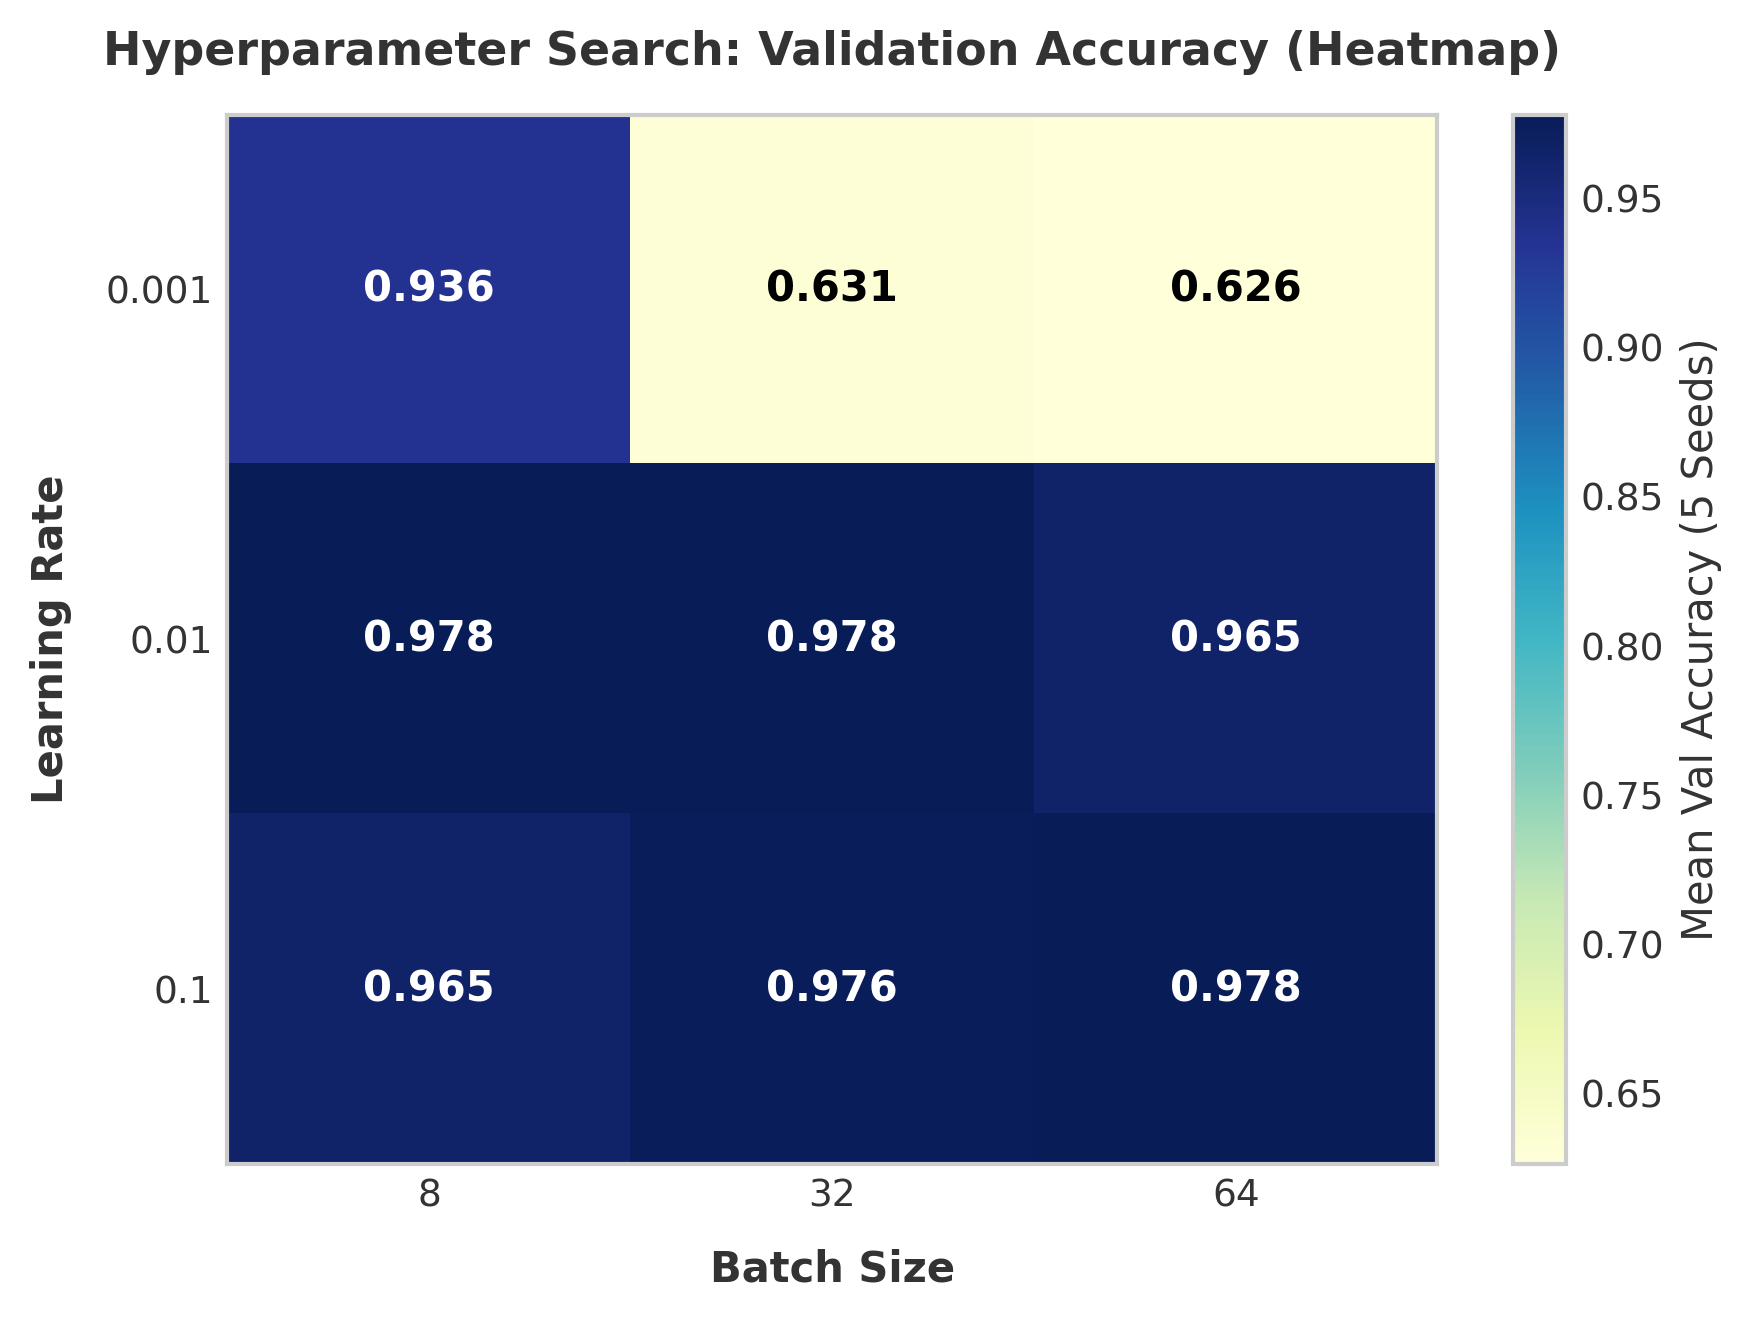
\includegraphics[width=0.75\linewidth]{hyperparam_heatmap.png}
    \caption{Heatmap de val acc ($\alpha \times$ \texttt{batch}).}
    \label{fig:heatmap}
\end{figure}

A Figura~\ref{fig:hypercurves} evidencia a \textbf{fase de latência}: curvas iniciam em $\approx$62,7\% ($357/569$ benignos) enquanto pesos pequenos e ReLUs inativas impedem quebra de simetria. Latência: $\alpha=0{,}1$ $\approx$2 épocas; $\alpha=0{,}01$ $\approx$18; $\alpha=0{,}001$ não sai do platô; \texttt{batch=8} mais rápido que 64; rede \texttt{[30,64,32,2]} $\approx$45 épocas.

\begin{figure}[H]
    \centering
    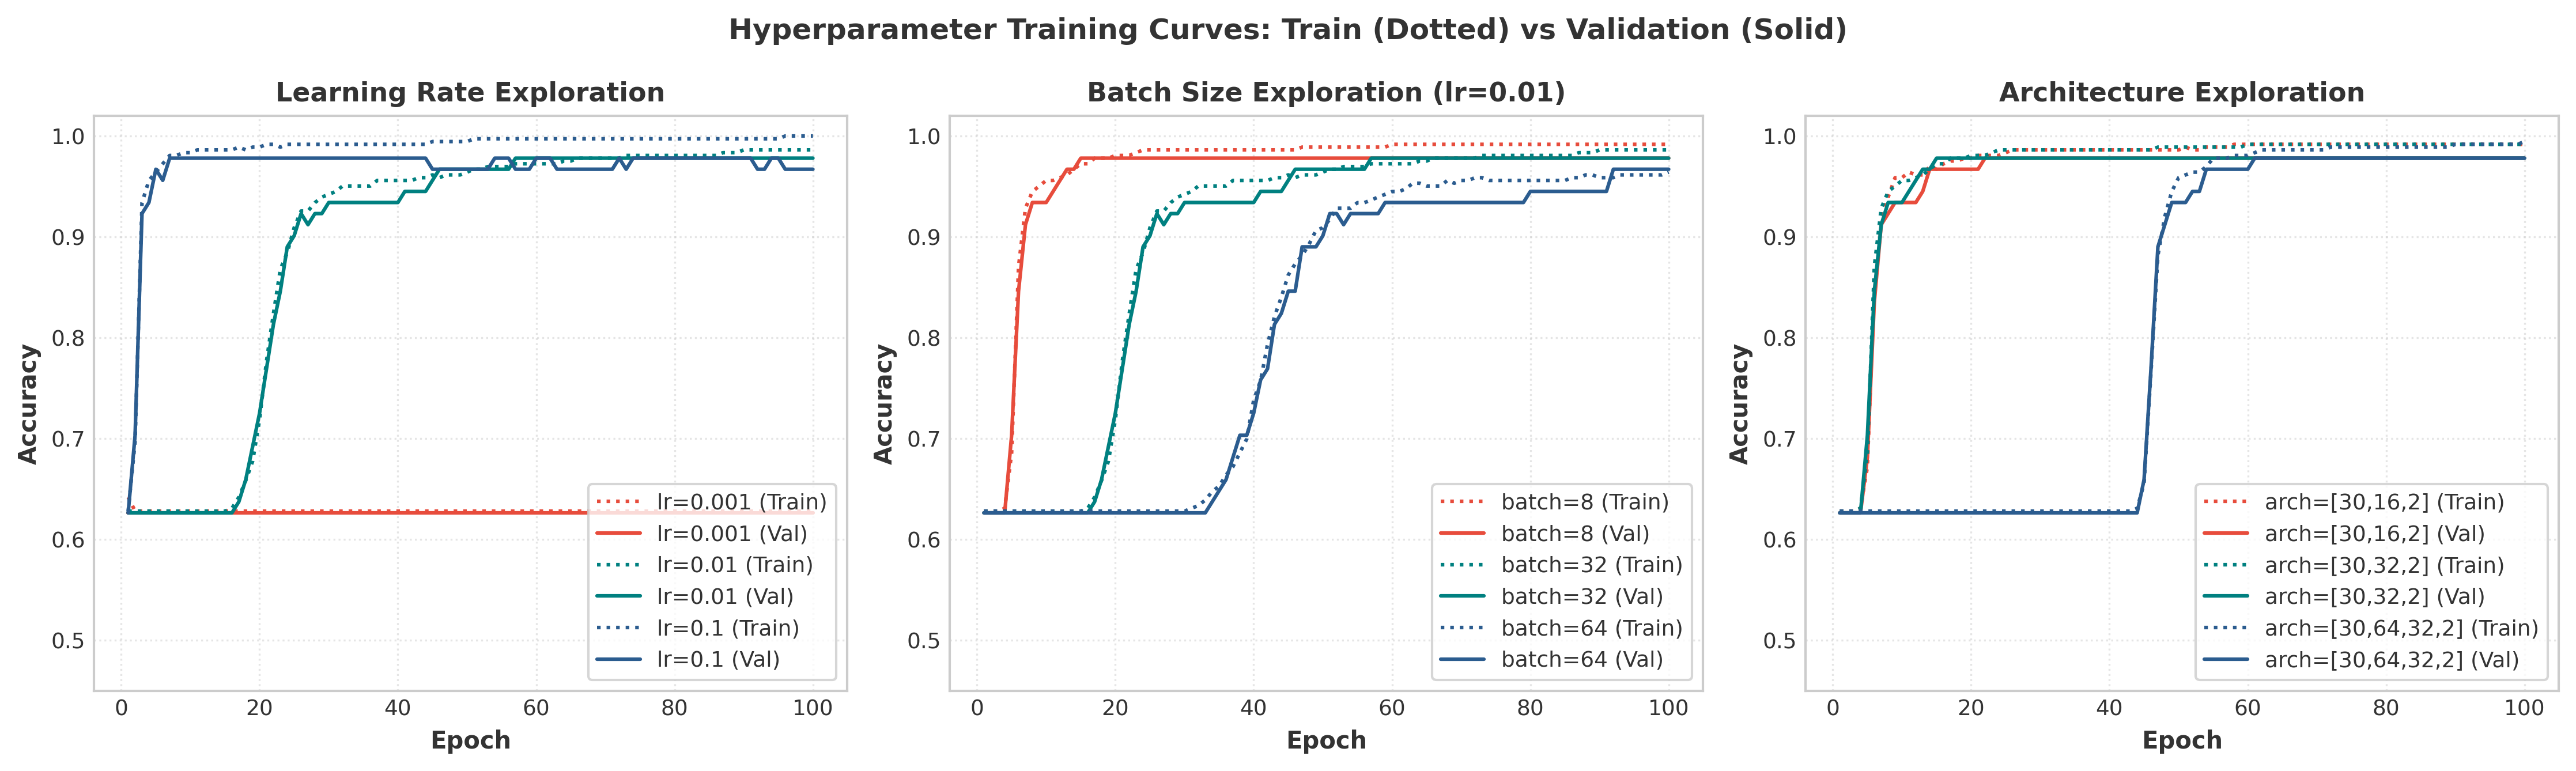
\includegraphics[width=0.95\linewidth]{hyperparam_training_curves.png}
    \caption{Curvas de acurácia ao variar $\alpha$, \texttt{batch} e arquitetura (treino pontilhado, validação sólida).}
    \label{fig:hypercurves}
\end{figure}

\subsection{Treinamento final e comparação \emph{shallow/deep}}

Adotamos \textbf{early stopping} em duas fases: (1) treinar em treino+validação separados por 200 épocas e identificar a época de menor val loss (época~37, loss 0{,}108); (2) retreinar em treino$\cup$validação (454 amostras) por exatamente 37 épocas e avaliar o teste uma vez.

\section{Resultados}

\textbf{Teste final:} acurácia \textbf{98,2\%} (112/114 corretos), test loss 0{,}085. A Figura~\ref{fig:confusion} mostra a matriz de confusão.

\begin{figure}[H]
    \centering
    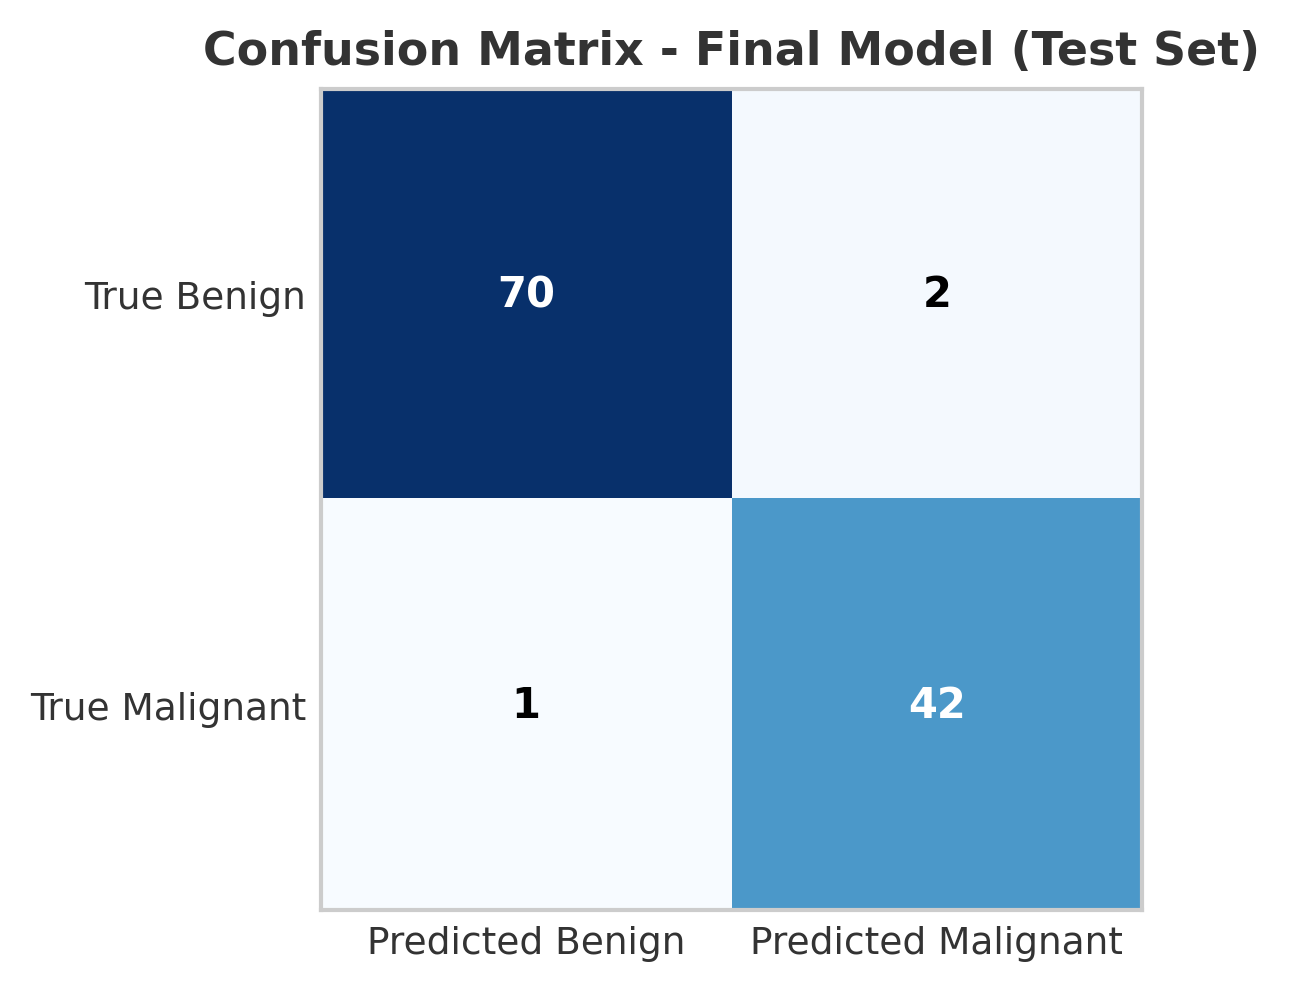
\includegraphics[width=0.42\linewidth]{final_test_confusion_matrix.png}
    \caption{Matriz de confusão no conjunto de teste final (0 = benigno, 1 = maligno).}
    \label{fig:confusion}
\end{figure}

Dois falsos negativos (malignos classificados como benignos) e nenhum falso positivo. Sensibilidade para malignos: 41/43 $\approx$ 95,3\%; especificidade: 71/71 = 100\%.

\textbf{Rede rasa vs.\ profunda:} em val acc as três arquiteturas empatam (0{,}978), mas a profunda exige muito mais épocas para sair do platô (Figura~\ref{fig:hypercurves}) e apresenta maior train acc (0{,}995), sugerindo capacidade extra não aproveitada neste dataset tabular pequeno. Optamos pela rede \texttt{[30,16,2]} por parsimônia.

\textbf{Extras omitidos por brevidade:} no notebook também comparamos \texttt{MLPClassifier} (sklearn), com mesma test acc (98,2\%), e avaliamos inicialização He e momentum (Seção~7), que encurtam a fase de latência; as figuras correspondentes ficam no repositório, mas foram omitidas aqui pelo limite de 6 páginas.

\section{Interpretabilidade}

Analisamos o \texttt{final\_model} por gradientes de entrada e ablação. Também implementamos SHAP (Seção~9 do notebook); omitimos essa análise aqui por brevidade e limite de páginas. Os \emph{summary plots} e \emph{waterfalls} SHAP estão em \texttt{figures/shap\_summary.png}.

\subsection{Importância global}

\textbf{Gradientes de entrada (6.1):} para cada amostra de teste, calculamos $\partial P(\hat{c})/\partial x_j$ em relação à classe predita e médiamos $|\partial P / \partial x_j|$. Features \texttt{worst\_*} dominam o ranking (e.g.\ \texttt{worst concave points}, \texttt{worst radius}, \texttt{worst texture}, \texttt{worst area}).

\textbf{Ablação (6.2):} zeramos features (individual, por família \texttt{mean\_*}/\texttt{worst\_*}/\texttt{*\_error}, ou por atributo-base) e medimos aumento de cross-entropy. Com apenas 114 amostras de teste, queda de acurácia é \textbf{discreta} (passos de $1/114 \approx 0{,}0088$), tornando \texttt{accuracy\_drop} pouco discriminante. Ranqueamos por \textbf{ce\_increase} e \textbf{true\_conf\_drop}.

\begin{itemize}
    \item \textbf{Feature individual:} \texttt{worst texture} (CE +0{,}012), \texttt{worst symmetry} (+0{,}009), \texttt{worst concavity} (+0{,}006).
    \item \textbf{Família:} \texttt{worst\_*} (+0{,}107 CE) $\gg$ \texttt{mean\_*} (+0{,}014) $\gg$ \texttt{*\_error} (+0{,}011).
    \item \textbf{Atributo-base:} \texttt{texture} (+0{,}030) lidera; \texttt{concavity} e \texttt{symmetry} seguem empatados em CE.
\end{itemize}

\textbf{Discordância entre métodos:} gradientes e ablação por feature coincidem parcialmente em \{\texttt{worst area}, \texttt{worst concave points}, \texttt{worst radius}, \texttt{worst texture}\}, mas a ablação por \emph{atributo-base} destaca \texttt{texture} enquanto gradientes enfatizam \texttt{concave points}. Essa divergência é esperada: gradientes medem sensibilidade local; ablação mede efeito global de remoção.

\subsection{Explicações individuais}

Waterfalls por gradiente$\times$input (Seção~6.3; figuras em \texttt{figures/waterfall\_patient\_*.png}, omitidas aqui):

\textbf{Paciente \#0} (benigno, $P(M)=0{,}396$, acerto): sinais conflitantes. \texttt{worst concave points} alto empurra maligno, mas \texttt{worst smoothness} compensa para benigno.

\textbf{Paciente \#2} (maligno, $P(M)=0{,}992$, acerto): caso ``fácil''; \texttt{worst texture/radius} elevados alinham-se com maligno.

\textbf{Paciente \#39} (benigno, $P(M)=0{,}602$, \textbf{falso positivo}): \texttt{mean radius} e \texttt{worst symmetry} empurram maligno; \texttt{worst radius/concavity} puxam benigno. Trata-se de sinal misto na região de overlap do PCA (Figura~\ref{fig:pca}).

\section{Discussão crítica}

\textbf{Limitações metodológicas:}
\begin{enumerate}
    \item \textbf{Teste pequeno (114 amostras):} métricas de ablação por acurácia são grosseiras; preferimos CE contínua, mas incertezas permanecem elevadas.
    \item \textbf{Validação estreita (91 amostras):} empates frequentes entre configs (val acc 0{,}978); escolhemos parsimônia, não superioridade estatística comprovada.
    \item \textbf{Early stopping + retreino:} embora evitemos \emph{peek} direto no teste durante busca de hiperparâmetros, o número de épocas ótimo foi estimado na validação; retreino em treino+val melhora robustez, mas não elimina variância de \emph{seed}.
    \item \textbf{Interpretabilidade:} gradientes pontuais e ablação binária (zerar feature) não capturam interações não-lineares; SHAP foi implementado mas omitido do relatório (ver notebook).
\end{enumerate}

\textbf{O que faríamos diferente:} validação cruzada $k$-fold para seleção de hiperparâmetros; regularização L2 explícita na rede profunda; calibração de probabilidades; técnicas mais suaves (Integrated Gradients); e exportar as curvas de early stopping para o relatório.

\textbf{Conclusão:} a MLP manual atinge desempenho comparável ao \texttt{MLPClassifier}, com interpretabilidade consistente no domínio clínico. Medidas \texttt{worst\_*} e morfologia de concavidade/textura são os preditores mais salientes, mas métodos de explicação devem ser lidos em conjunto, não isoladamente.

\begin{thebibliography}{9}
\bibitem{sklearn-bc}
Pedregosa et al. Scikit-learn: \emph{Breast Cancer Wisconsin (Diagnostic) Dataset}. \url{https://scikit-learn.org/stable/datasets/toy_dataset.html#breast-cancer-dataset}
\end{thebibliography}

\end{document}
